\section{Onocoy as the Anchor Case}
\label{sec:onocoy_anchor_case}

Onocoy functions as the empirical anchor for this thesis because it combines three features that are analytically useful together: a hardware-dependent DePIN service, a capped-supply token design, and a dual-layer payment architecture that separates user-facing service pricing from direct token volatility. That combination gives us a strong case for asking how infrastructure quality, user demand, and token-side incentives interact when stress enters a network that cannot rely on purely digital capital mobility.

We do not treat Onocoy as a proxy for the whole DePIN landscape. We use the case more narrowly. Onocoy provides a documented mechanism design that can be described with enough clarity to support the later empirical and methodological chapters, while still exposing the kinds of documentation gaps and design tradeoffs that matter for a bounded stress-evaluation thesis.

\subsection{System Function and Network Participants}
Onocoy operates a decentralized GNSS correction network based on Real-Time Kinematic (RTK) positioning. RTK combines correction data from reference stations with rover-side measurements in order to improve positioning accuracy from meter-scale error bands toward centimeter-level precision, which matters for surveying, precision agriculture, robotics, and industrial workflows where positional error is operationally costly \cite{OnocoyWhitepaper301}.

The network depends on geographically distributed reference stations rather than on a single centralized infrastructure operator. In practical terms, this means that the quality of the system depends not only on whether stations exist, but on where they are installed, how reliably they remain online, and whether their correction output is usable within the network's service layer \cite{OnocoyWhitepaper301}. That makes Onocoy analytically useful for this thesis because it sits inside an already established GNSS ecosystem: instead of inventing demand from nothing, it inserts a decentralized correction layer into positioning workflows that already care about continuity, precision, and coverage quality.

That creates two primary participant groups. First, reference-station operators deploy and maintain GNSS hardware, connectivity, and quality-relevant uptime. Their role is not passive. Installation quality, calibration, and maintenance discipline affect the usefulness of the correction data they contribute \cite{OnocoyWhitepaper301, OnocoyRewards}. Second, rover-side users purchase correction access for high-accuracy positioning tasks. In the Onocoy case, the expected demand profile is closer to professional or industrial usage than to purely narrative retail usage, which makes continuity, measured quality, and coverage density central to the service proposition \cite{OnocoyWhitepaper301}.

Onocoy's public Explorer adds an operational transparency layer to that service model. The explorer does not only display that stations exist; it visualizes a coverage heatmap and exposes station-level details such as approximate validated location, validation status, uptime, signals, quality scale, and estimated rewards \cite{OnocoyExplorer}. For this thesis, that matters because it makes the network spatially tangible: users and operators can observe where coverage is already dense, where overlap exists, and where additional stations may improve useful correction availability.

Separate from the thesis interview process, the Onocoy ecosystem also appears to include an active community-support layer around operators. Public documentation describes ambassador and community channels that support ecosystem participation, while bounded practitioner context suggests these spaces are also used to exchange installation practices, reward information, and deployment feedback \cite{OnocoyAmbassador}. This thesis treats that layer as ecosystem context rather than as a mechanism fact, but it still helps explain why participation in a GNSS DePIN is operationally richer than simply switching a device on and waiting for rewards.

\subsection{Token and Payment Architecture}
Onocoy uses a dual-layer design with ONO as the transferable utility and governance token, while Data Credits function as the non-transferable unit for service consumption. Official tokenomics documentation describes ONO as a capped utility token with a maximum supply of 810 million units, while Data Credits are purchased against fiat-denominated value and then consumed during network use \cite{OnocoyWhitepaper301, OnocoyToken, OnocoyTokenomics}. That separation matters because it allows the immediate user-side service price to remain more stable than the market price of ONO itself.

This architecture matters because it separates two questions that are often blurred in simpler token systems. The first is whether users face a predictable service price. The second is whether the protocol still creates a credible path from service demand back into token-side support. In the documented flow, users prepay for service through Data Credits, those credits are burned when GNSS data services are consumed, and the resulting fiat revenue finances operations and may also be used for ONO buybacks. The tokenomics documentation further states that bought-back ONO can be split across the reward pool, ecosystem pool, and token burn \cite{OnocoyTokenomics}. For the reader, the important point is not only that ONO and Data Credits are different units. It is that pricing, service consumption, and token-side settlement are separated enough to shield the user from direct token volatility while still keeping demand economically relevant to the incentive system.

Public Onocoy documentation therefore supports three mechanism facts particularly clearly: a capped ONO supply, a release path described as a 16\% annual reduction in newly distributed units, and a Data Credit layer whose use is tied to burn and conditional buyback routing \cite{OnocoyWhitepaper301, OnocoyTokenomics}. That makes the payment architecture unusually important to the case. If the user-facing credit layer creates stability but the routing back into token-side support is too weak, the network can still face stress on the supply side even when users see a smoother service price.

\begin{figure}[H]
    \centering
    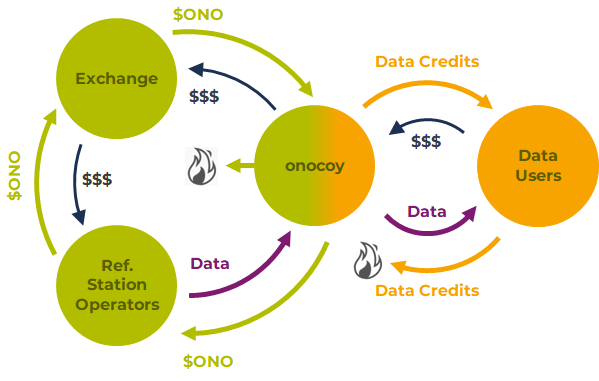
\includegraphics[width=0.82\textwidth]{figures/onocoy_token_flow_docs.png}
    \caption[Onocoy tokenomics flow]{Official Onocoy tokenomics flow, showing how ONO, Data Credits, data users, exchange liquidity, and reference-station operators interact in the public design description \cite{OnocoyTokenomics}.}
    \label{fig:v2_onocoy_token_flow}
\end{figure}

The public-doc picture is stronger for ONO issuance and Data Credit mechanics than for every operational participation detail. For this thesis, that distinction matters. Emission and payment architecture can be described as mechanism facts. At the same time, the current public design does not center participation on an explicit staking- or collateral-based miner model. Where later chapters require assumptions, they arise from other operational unknowns rather than from a missing stake-based participation layer \cite{OnocoyToken, OnocoyRewards}.

\begin{table}[H]
    \centering
    \small
    \renewcommand{\arraystretch}{1.2}
    \begin{tabularx}{\textwidth}{@{}p{0.30\linewidth}X@{}}
        \toprule
        \textbf{Dimension} & \textbf{Onocoy case summary} \\
        \midrule
        Infrastructure domain & Decentralized GNSS correction network using RTK positioning services. \\
        Provider role & Reference-station operators deploy and maintain GNSS hardware, connectivity, and quality-relevant uptime. \\
        Demand side & Rover-side users purchase correction access for professional and industrial positioning workflows. \\
        Token / credit architecture & Transferable ONO token plus non-transferable Data Credits used for service consumption. \\
        User-side pricing logic & Data Credits are priced against fiat-denominated value rather than exposing users directly to ONO market volatility. \\
        Supply-side release path & Public documentation describes capped ONO supply with a decaying distribution path. \\
        Documentation boundary & Public materials are explicit about ONO and Data Credit mechanics and do not present a staking- or collateral-based participation model; the thinner areas lie in other operational participation details. \\
        \bottomrule
    \end{tabularx}
    \caption[Onocoy case summary]{Onocoy case summary used as the thesis anchor case.}
    \label{tab:v2_onocoy_case_summary}
\end{table}

\subsection{Settlement-Layer Scope and Decision Boundary}
We treat Onocoy's blockchain choice as a settlement-layer design decision tied to timing, throughput and cost requirements, and off-chain service delivery constraints rather than as a general claim that one chain is universally superior. The practical requirement in scope is straightforward: the network must support frequent, low-value accounting events while keeping latency-sensitive GNSS correction delivery off-chain for operational reasons \cite{OnocoyWhitepaper301, OnocoyToken}.

That decision is best understood in the project window in which many DePIN teams were choosing between operating sovereign chain infrastructure and deploying into an existing settlement ecosystem. Published chain-selection material for Onocoy describes a structured screening funnel and links the final choice to throughput, cost, block-time expectations, ecosystem readiness, and engineering execution constraints during that decision period \cite{Ballandies2023ChainSelection}. In this chapter, we use those factors as project-primary evidence for a time-bounded architecture choice, not as a timeless benchmark for all future DePINs.

For Onocoy specifically, the practical advantage is not abstract chain branding. It is operational fit. A settlement layer with relatively low transaction cost and high-frequency processing makes it easier to meter small-value service usage, support fine-grained accounting, and avoid turning the economic layer into a bottleneck for either providers or users.

On the supply side, that reduces friction around recurring reward accounting and token-side settlement. On the demand side, it supports a service model in which pricing and access can be broken down more granularly than a slower or more expensive chain would comfortably permit. In that sense, settlement-layer choice becomes part of DePIN mechanism viability rather than a purely backend engineering preference.

The broader industry context reinforces that bounded reading. A DePIN project can either build and maintain dedicated chain infrastructure or use an existing settlement environment while concentrating product effort on service delivery and mechanism operations. Helium's migration record is relevant here as contextual evidence that chain-maintenance burden can compete directly with product-layer execution capacity, but it is not treated as proof that Onocoy's own choice is universally optimal \cite{HeliumHIP70}. More generally, DePIN projects are forced to make execution-layer tradeoffs under the constraints of their own era, product requirements, and ecosystem options. That is why this thesis treats Onocoy's chain choice as a historically situated design decision rather than as a universal model for every later DePIN.

\subsection{Case Relevance, Documentation Gaps, and Evidence Boundary}
Onocoy matters to this thesis because it narrows the comparative framework developed in Chapter~\ref{sec:comparative_tokenomic_framework} into a concrete capped-supply design that still depends on physical infrastructure quality, measurable service demand, and token-side coordination. The case is especially useful because the project does not only present a token architecture. It also exposes how difficult it is to document every relevant participation rule with equal clarity once a DePIN begins to combine off-chain service delivery, quality-sensitive hardware, and on-chain economic settlement.

We have to handle that asymmetry in documentation explicitly. Public sources are sufficiently clear to support claims about RTK service function, the dual-layer ONO/Data Credit design, and the general supply-decay path. They also indicate that the current public design is not framed around staking or collateral participation. The thinner areas lie elsewhere. Some operational participation details remain less explicit than the token and payment architecture itself. Where those items matter later, they must be treated either as unknown mechanism facts or as declared modeled assumptions rather than as silently completed facts.

The same discipline applies to the Explorer, to Dune, and to the interview material used in this thesis, but for different reasons. In this chapter, we treat the Explorer as an operational and spatial transparency layer: it shows coverage, station-level quality signals, and deployment geography. Dune, by contrast, is used as a public on-chain analytics layer that can support dated, auditable snapshots of selected token-side and activity-side indicators \cite{OnocoyExplorer, OnocoyDuneDashboard}. The point of using a dated Dune snapshot here is not to prove growth, robustness, or long-run trend. It is to show which layers of the Onocoy case are publicly visible before the thesis later asks what can be observed empirically and what must instead be handled through bounded evaluator logic.

\begin{table}[H]
    \centering
    \small
    \renewcommand{\arraystretch}{1.2}
    \begin{tabularx}{\textwidth}{@{}>{\raggedright\arraybackslash}p{0.24\linewidth}>{\raggedright\arraybackslash}p{0.28\linewidth}X@{}}
        \toprule
        \textbf{Observable Layer} & \textbf{Snapshot Values (25 February 2026)} & \textbf{What the Snapshot Makes Visible} \\
        \midrule
        Token-holder and supply visibility & 1{,}568 holders; 75{,}713{,}648 circulating ONO & Shows that token-side participation and circulating supply are at least partly visible through public accounting surfaces rather than entirely hidden from the analysis. \\
        \midrule
        Buyback and burn accounting & 2{,}928{,}777 total ONO buybacks; 2{,}024{,}536 total ONO burned & Shows that some sink- and treasury-related token flows can be observed directly enough to support dated descriptive claims about the settlement layer. \\
        \midrule
        Participation-side network visibility & 7{,}668 validated stations; 5{,}638 online stations & Shows that network participation is visible not only as a token system, but also as a live infrastructure layer with measurable validated and online station counts. \\
        \bottomrule
    \end{tabularx}
    \caption[Onocoy Dune observability anchor]{Dated Dune observability anchor for Onocoy on 25 February 2026.}
    \label{tab:v2_onocoy_dune_anchor}
\end{table}

This snapshot anchors observability rather than performance. It shows that some token-side, accounting-side, and participation-side fields are publicly visible at a defined point in time, while other economically important dimensions remain much less settled. On its own, it cannot establish trend direction or resolve questions such as revenue depth, churn history, or client concentration. That asymmetry is part of what makes Onocoy analytically useful as an anchor case.

The thesis also includes bounded interview-based practitioner context, while the public ambassador and community material is treated separately as ecosystem context rather than as a mechanism description. We use the interview layer to identify documentation gaps, clarify how operators and the project team describe practical conditions, and surface where public materials are thinner than the mechanism would ideally require. It does not carry the same evidentiary weight as protocol documentation or directly auditable public artifacts, and it is not treated here as a substitute for them.

Taken together, the public documentation, official tokenomics description, Explorer visibility layer, dated Dune snapshots, bounded interview context, and ecosystem-community layer make Onocoy especially relevant to the thesis. The case is documented enough to describe clearly, operational enough to visualize concretely, and incomplete enough to make evidence discipline visible rather than optional. That combination is precisely what makes it a useful anchor before the thesis turns to empirical observability limits and then to the narrower logic of DTSE.
